\begin{frame}
	\frametitle{Bref historique}
	\only<1>{
		\paraTitle{Sur le boosting}
		\begin{itemize}
			\itemperso{1989}Boosting (R. Schapire)
			\itemperso{1996}AdaBoost (Y. Freund et R. Schapire)
			\itemperso{1999}GBM (L. Breiman puis J. Friedman)
			\itemperso{2014}XGBoost (T. Chen)
		\end{itemize}
	}
	\only<2->{
		\paraTitle{Pour XGBoost}
		\begin{itemize}
	}
		\only<2->{
			\itemperso{Mars 2014}Première release
			\itemperso{Mai 2014}Python
		}
		\only<3->{
			\itemperso{Septembre 2014}Parallélisation, R
			\itemperso{Mai 2015}YARN, gestion HDFS, SKLearn wrapper
		}
		\only<4->{
			\itemperso{Janvier 2016}API JAVA, Flink, Spark, améliorations
			\itemperso{Juillet 2016}Totale compatibilité JVM (Spark,...)
		}
	\only<2->{
		\end{itemize}\vspace*{\fill}
	}
	\only<2>{
		\rule{0pt}{0pt}\hfill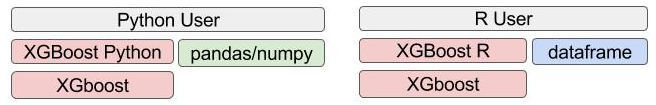
\includegraphics[width=.8\textwidth]{images/implementation/v1}\hfill\rule{0pt}{0pt}
	}
	\only<3>{
		\rule{0pt}{0pt}\hfill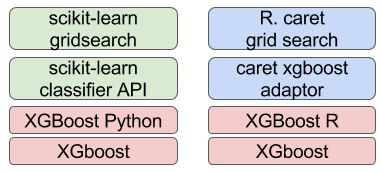
\includegraphics[width=.6\textwidth]{images/implementation/v2}\hfill\rule{0pt}{0pt}
	}
	\only<4>{
		\rule{0pt}{0pt}\hfill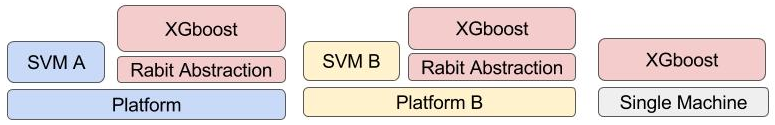
\includegraphics[width=.8\textwidth]{images/implementation/v3}\hfill\rule{0pt}{0pt}
	}
	\only<2->{
		\vspace*{\fill}\rule{0pt}{0pt}

		\rule{0pt}{0pt}\hfill{\fontsize{.15cm}{0cm}\selectfont{\textit{Source : \texttt{http://homes.cs.washington.edu/\textasciitilde tqchen/2016/03/10/story-and-lessons-behind-the-evolution-of-xgboost.html}}}}
	}
\end{frame}

\begin{frame}
	\frametitle{Trois familles de paramètres}
	\paraTitle{Paramètres génériques}
	
	Pour définir par exemple quelle méthode Boosting sera utilisée.
	
	\paraTitle{Paramètres liés au Boosting}
	
	Pour paramétrer le booster choisi.
	
	\paraTitle{Paramètres liés à l'apprentissage}
	
	Dépend de la tâche d'apprentissage (classification,...).
\end{frame}

\begin{frame}
	\frametitle{Paramètres génériques}
	\begin{itemize}
		\itemperso{\texttt{Booster}}Linéaire ou arbre.\vspace*{.2cm}
		\itemperso{\texttt{Silent}}Affichage de messages.\vspace*{.2cm}
		\itemperso{\texttt{Nthread}}Par défaut le maximum possible.\vspace*{.2cm}
	\end{itemize}
\end{frame}

\begin{frame}
	\frametitle{Paramètres liés au Boosting}
	\textit{Pour celui sur les arbres. Douze paramètres utiles...}\vspace*{.2cm}

	\begin{itemize}
		\itemperso{\texttt{Eta}}Contrôle du niveau d'apprentissage.
		\itemperso{\texttt{Min\_child\_weight}}Pour contrôler l'over/under-fitting
		\itemperso{\texttt{Max\_depth}}Pour contrôler l'over-fitting.
		\itemperso{\texttt{Lambda}}Pour de la régularisation.
		\itemperso{\texttt{Gamma}}Valeur minimale de gain pour diviser.
		\itemperso{...}
	\end{itemize}
\end{frame}

\begin{frame}
	\frametitle{Paramètres liés à l'apprentissage}
	\begin{itemize}
		\itemperso{\texttt{Objective}}Fonction objectif à minimiser (linéaire, softmax, softprob,...).\vspace*{.2cm}
		\itemperso{\texttt{Eval\_metric}}Métrique d'évaluation (erreur MSE, MAE, LogLoss, AUC,...).\vspace*{.2cm}
		\itemperso{\texttt{Seed}}Pour l'aléatoire.\vspace*{.2cm}
	\end{itemize}
\end{frame}

\begin{frame}[fragile]
	\frametitle{Utilisation avec Spark et Scala}
	\begin{lstlisting}[language=Scala]
val spark = SparkSession.builder().appName("SimpleXGBoost Application").config("spark.executor.memory", "2G").config("spark.executor.cores", "4").config("spark.default.parallelism", "4").master("local[*]").getOrCreate()

// number of iterations
val numRound = 10
val numWorkers = 4
// training parameters
val paramMap = List(
      "eta" -> 0.023f,
      "max_depth" -> 10,
      "min_child_weight" -> 3.0,
      "subsample" -> 1.0,
      "colsample_bytree" -> 0.82,
      "colsample_bylevel" -> 0.9,
      "base_score" -> 0.005,
      "eval_metric" -> "auc",
      "seed" -> 49,
      "silent" -> 1,
      "objective" -> "binary:logistic").toMap
println("Starting Xgboost ")
val xgBoostModelWithDF = XGBoost.trainWithDataFrame(trainingData, paramMap,round = numRound, nWorkers = numWorkers, useExternalMemory = true)

val predictions = xgBoostModelWithDF.setExternalMemory(true).transform(testData).select("label", "probabilities")\end{lstlisting}
\end{frame}

\begin{frame}[fragile]
	\frametitle{R et fonction de perte personnalisée}
	\begin{lstlisting}[language=R]
loglossobj <- function(preds, dtrain) {
  # dtrain is the internal format of the training data
  # We extract the labels from the training data
  labels <- getinfo(dtrain, "label")
  # We compute the 1st and 2nd gradient, as grad and hess
  preds <- 1/(1 + exp(-preds))
  grad <- preds - labels
  hess <- preds * (1 - preds)
  # Return the result as a list
  return(list(grad = grad, hess = hess))
}

model <- xgboost(data = train$data, label = train$label,
             nrounds = 2, objective = loglossobj, eval_metric = "error")\end{lstlisting}
\end{frame}

\begin{frame}[fragile]
	\frametitle{Sélection de variables}
	\begin{lstlisting}[language=R]
bst <- xgboost(data = train$data, label = train$label, max.depth = 2,
           eta = 1, nthread = 2, nround = 2,objective = "binary:logistic")
importance_matrix <- xgb.importance(agaricus.train$data@Dimnames[[2]], model = bst)
xgb.plot.importance(importance_matrix)\end{lstlisting}
	\begin{center}
		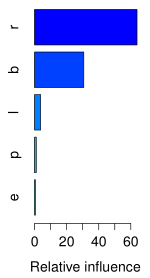
\includegraphics[width=.25\textwidth]{images/implementation/importance}
	\end{center}
	\rule{0pt}{0pt}\hfill{\fontsize{.15cm}{0cm}\selectfont{\textit{Source : \texttt{http://dmlc.ml/rstats/2016/03/10/xgboost.html} et cours d'apprentissage statistique (C. \textsc{Helbert})}}}	
\end{frame}

\begin{frame}
	\frametitle{Quelques bonnes pratique}
	\begin{itemize}
		\itemperso{1.}Fixer un niveau d'apprentissage élevé.\vspace*{.2cm}
		\itemperso{2.}Trouver le nombre optimal d'arbres.\vspace*{.2cm}
		\itemperso{3.}Gérer les paramètres des arbres.\vspace*{.2cm}
		\itemperso{4.}Gérer les paramètres de régularisation.\vspace*{.2cm}
		\itemperso{5.}Réduire le niveau d'apprentissage.\vspace*{.2cm}
		\itemperso{6.}Utiliser l'AUC pour estimer les modèles.\vspace*{.2cm}
	\end{itemize}
\end{frame}